% Dies ist die Hauptdatei, von der aus das Gesamtdokument erzeugt wird.  Diese
% Datei sollten Sie zunächst umbenennen, damit sie keinen generischen Namen
% hat!  Dann wird sie mit LuaLaTeX kompiliert.

% In der Datei defs.tex werden alle globalen LaTeX-spezifischen Einstellungen
% vorgenommen
% Jede LaTeX-Datei beginnt mit der Dokumentenklasse.  Für diese Vorlage wurde
% die Klasse "scrreprt" von KOMA-Script gewählt, die in etwa der
% Standardklasse "report" entspricht, allerdings wesentlich mehr Möglichkeiten
% bietet und im gewissen "moderner" ist.  Eine sehr ausführliche Dokumentation
% zu KOMA-Script findet man unter der folgenden Adresse:
% http://mirrors.ctan.org/macros/latex/contrib/koma-script/doc/scrguide.pdf
\documentclass[
  % die Schriftgröße - sollten Sie nicht ändern
  fontsize=12pt,
  % das Papierformat, also DIN A4
  paper=A4,
  % Literaturverzeichnis ins Inhaltsverzeichnis
  bibliography=totoc,
  % andere Verzeichnisse ebenfalls ins Inhaltsverzeichnis
  listof=totoc,
  % abgesetzte Formeln linksbündig
  fleqn,
  % für die Satzspiegelkonstruktion - siehe KOMA-Doku
  DIV=12,
  % Bindekorrektur (linker Rand) - evtl. anpassen
  BCOR=1mm,
  % die im Text verwendeten Sprachen (u.a. für das Paket babel); die
  % letztgenannte (!) Sprache ist die Standardsprache; "n"german steht für die
  % neue Rechtschreibung
  english,ngerman,
  % weil (s.u.) das Paket geometr verwendet wird
  usegeometry,
  % wie Absätze gesetzt werden: ohne Einzug, halbe Zeile Abstand
  parskip=half-
]{scrreprt}

% Beschriftungen für Tabellen kommen linksbündig über die Tabelle
\KOMAoption{captions}{tableheading,nooneline}
\setcaptionalignment[figure]{c}
\setcaptionalignment[table]{l}

% wird für die Titelseite benötigt
\usepackage{geometry}

% Standardpaket für Lokalisation, siehe Option "ngerman" oben
\usepackage{babel}
% Laden von optimierten Trennmustern
\babelprovide[hyphenrules=ngerman-x-latest]{ngerman}

% Standardpaket für mathematische Zusatzfunktionen; wenn Sie keine
% mathematischen Formeln brauchen, können Sie diese Zeile löschen
\usepackage{amsmath}

% die Hauptschrift Libertinus
\usepackage{libertinus-otf}
% die "Schreibmaschinenschrift" Anonymous Pro, angepasst
\usepackage{AnonymousPro}
\setmonofont{AnonymousPro}[Scale=MatchLowercase,FakeStretch=0.85]

% etwas größerer Zeilenabstand als im Buchsatz
\linespread{1.1}

% Paket für Feinkorrekturen an der Typographie, das für ein ausgewogeneres
% Schriftbild sorgt
\usepackage{microtype}

% Paket für kontextsensitive Anführungszeichen
\usepackage{csquotes}
% Shortcut, damit aus dem eigentlich falschen Zeichen " richtige
% Anführungszeichen je nach Sprache werden
\MakeOuterQuote{"}

% Paket, das den Befehl \includegraphics ermöglicht
\usepackage{graphicx}

% komfortablere Aufzählungen als in Standard-LaTeX; ein Beispiel findet man in
% chap3.tex
\usepackage{enumitem}

% Paket für mehr als die üblichen Standardfarben
\usepackage[dvipsnames]{xcolor}
% Definition der "Hausfarben" der HAW
\definecolor{haw}{HTML}{003CA0}
\definecolor{haw2}{HTML}{0096D2}
\definecolor{haw3}{HTML}{A0BEDC}
\definecolor{darkgreen}{rgb}{0, 0.5, 0}
\definecolor{background}{HTML}{EEEEEE}
\definecolor{delim}{RGB}{20,105,176}
\colorlet{punct}{red!60!black}
\colorlet{numb}{magenta!60!black}

% typographisch anspruchsvolle Tabellen; siehe chap3.tex
\usepackage{booktabs}

% zum Erstellen des Literaturverzeichnisses; der gängige Stil APA ist hier
% bereits eingestellt
\usepackage[style=apa]{biblatex}
% eine Beispieldatei für ein Literaturverzeichnis
\addbibresource{bachelorarbeit.bib}

% für die Erzeugung der Grafiken in chap3.tex; wenn Sie PGF/TikZ nicht
% verwenden wollen, können Sie diese Zeilen entfernen
\usepackage{tikz}
% Zusatzbibliotheken für TikZ, die in den genannten Beispielen verwendet
% werden
\usetikzlibrary{calc,intersections,angles,3d}

% für die Erzeugung des Codeblocks in chap3.tex; wenn in Ihrer Arbeit keine
% Codeblöcke vorkommen, können Sie diese Zeilen entfernen
\usepackage{listings}

% see https://tex.stackexchange.com/questions/83085/how-to-improve-listings-display-of-json-files
\lstdefinelanguage{json}{
    basicstyle=\normalfont\ttfamily,
    numbers=left,
    numberstyle=\scriptsize,
    stepnumber=1,
    numbersep=8pt,
    showstringspaces=false,
    breaklines=true,
    frame=lines,
    backgroundcolor=\color{background},
    literate=
    *{0}{{{\color{numb}0}}}{1}
        {1}{{{\color{numb}1}}}{1}
        {2}{{{\color{numb}2}}}{1}
        {3}{{{\color{numb}3}}}{1}
        {4}{{{\color{numb}4}}}{1}
        {5}{{{\color{numb}5}}}{1}
        {6}{{{\color{numb}6}}}{1}
        {7}{{{\color{numb}7}}}{1}
        {8}{{{\color{numb}8}}}{1}
        {9}{{{\color{numb}9}}}{1}
        {:}{{{\color{punct}{:}}}}{1}
        {,}{{{\color{punct}{,}}}}{1}
        {\{}{{{\color{delim}{\{}}}}{1}
        {\}}{{{\color{delim}{\}}}}}{1}
        {[}{{{\color{delim}{[}}}}{1}
        {]}{{{\color{delim}{]}}}}{1},
}
% see https://tex.stackexchange.com/questions/152829/how-can-i-highlight-yaml-code-in-a-pretty-way-with-listings
\newcommand\YAMLcolonstyle{\color{red}\mdseries}
\newcommand\YAMLkeystyle{\color{black}\bfseries}
\newcommand\YAMLvaluestyle{\color{blue}\mdseries}

\makeatletter

\newcommand\language@yaml{yaml}

\expandafter\expandafter\expandafter\lstdefinelanguage
\expandafter{\language@yaml}
{
    keywords={true,false,null,y,n},
    keywordstyle=\color{darkgray}\bfseries,
    basicstyle=\YAMLkeystyle,
    sensitive=false,
    comment=[l]{\#},
    morecomment=[s]{/*}{*/},
    commentstyle=\color{purple}\ttfamily,
    stringstyle=\YAMLvaluestyle\ttfamily,
    moredelim=[l][\color{orange}]{\&},
    moredelim=[l][\color{magenta}]{*},
    moredelim=**[il][\YAMLcolonstyle{:}\YAMLvaluestyle]{:},
    morestring=[b]',
    morestring=[b]",
    literate =    {---}{{\ProcessThreeDashes}}3
        {>}{{\textcolor{red}\textgreater}}1
        {|}{{\textcolor{red}\textbar}}1
        {\ -\ }{{\mdseries\ -\ }}3,
}

\lst@AddToHook{EveryLine}{\ifx\lst@language\language@yaml\YAMLkeystyle\fi}
\makeatother
\newcommand\ProcessThreeDashes{\llap{\color{cyan}\mdseries-{-}-}}

\lstdefinelanguage{math}{
    keywords={SIGNED, UNSIGNED},
    sensitive=true,
    morekeywords={bis},
    keywordstyle=\color{blue}\bfseries,
    comment=[l]\%,
    string=[b]",
    morestring=[b]',
    moredelim=*[s][\color{gray}]{/*}{*/},
    morekeywords={[2]Beispiel},
    keywordstyle={[2]\color{haw2}\bfseries},
}

% Anpassung des Erscheinungsbildes des Codeblocks; mehr dazu in der
% Dokumentation des Pakets "listings"
\lstdefinestyle{mystyle}{
    backgroundcolor=\color{gray!20},
    keywordstyle=\color{haw2},
    numberstyle=\footnotesize\color{haw},
    basicstyle=\ttfamily\small,
    captionpos=t,
    frame=single,
    framerule=0pt,
    keepspaces=true,
    numbers=left,
    numbersep=6pt,
    belowcaptionskip=1em,
    aboveskip=\bigskipamount,
}

\lstdefinestyle{custom_daniel}{
    backgroundcolor=\color{gray!20},
    basicstyle=\ttfamily\small,
    keywordstyle=\color{haw2},
    commentstyle=\color{gray},
    numberstyle=\footnotesize\color{haw},
    stringstyle=\color{darkgreen},
    numbers=left,
    breaklines=true,
    keepspaces=true,
    showspaces=false,
    showstringspaces=false,
}
\lstset{style=mystyle}
% damit es "Codeblock" und nicht "Listing" heißt
\renewcommand{\lstlistingname}{Codeblock}

% für die Verlinkung innerhalb des PDF-Dokuments, für PDF-Lesezeichen und
% PDF-Metadaten; dieses Paket sollte üblicherweise immer als letztes geladen
% werden
\usepackage[colorlinks=true,allcolors=haw,hyperfootnotes=false,pageanchor=true,linktoc=all]{hyperref}

% für die Druckversion können Sie die obige Zeile durch die folgende ersetzen,
% damit Links nicht blau dargestellt werden:
% \usepackage[draft]{hyperref}

% Metadaten des PDF-Dokumentes; setzen Sie hier Ihren eigenen Namen sowie den
% Titel Ihrer Arbeit ein
\hypersetup{pdfauthor={Daniel Freire Mendes}}
\hypersetup{pdftitle={Performance-Optimierung von Datenbanken}}

\usepackage{subcaption}
\usepackage{float}
\usepackage[labelfont=bf]{caption}

% Wenn das Kommentarzeichen entfernt wird, kann man mit einem Befehl wie
%
% \includeonly{chap2,chap3}
%
% erreichen, dass nur ausgewählte Dateien kompiliert werden.  Das ist für die
% Arbeit an umfangreichen Dokumenten hilfreich, weil es Zeit spart.  Für das
% Erstellen des fertigen Dokuments muss der Befehl natürlich wieder
% auskommentiert werden, damit alle Referenzen aktuell sind und die
% Seitenzahlen stimmen.

% Hier beginnt das eigentliche Dokument.  Sie können weitere Dateien
% hinzufügen und natürlich auch vorhandene weglassen.  Die vorhandene
% Dateistruktur ist lediglich als Beispiel gedacht.
\begin{document}
% In dieser Umgebung wird die Titelseite separat vom restlichen Text gesetzt
\begin{titlepage}
  % andere Seitenränder als im Rest der Arbeit
  \newgeometry{lmargin=2cm,tmargin=7mm,rmargin=5mm,bmargin=1cm}
  % die "Hausfarbe" der HAW; diese und die folgenden Einstellungen sind lokal
  % und gelten nur innerhalb der Umgebung "titlepage"
  \color{haw}
  % Blocksatz für die Titelseite deaktivieren
  \raggedright
  % Logo rechtsbündig setzen
  \hfill
\includegraphics[width=7cm]{PNGs/General/HAW_Marke_RGB_300dpi}\\

  % vertikaler Abstand
  \vspace{5cm}

  % Wahl der "Hausschrift" Open Sans der HAW, die als Schrift auf Ihrem
  % Rechner installiert sein muss
  \setmainfont{Open Sans}
  % etwas kleiner als üblich
  \small
  % fett und in Majuskeln
  \textbf{BACHELORARBEIT}

  % vertikaler Abstand
  \vspace{8mm}

  % der Titel der Arbeit als "Seite in der Seite"; natürlich müssen Sie hier
  % Ihren Titel eintragen
  \begin{minipage}{0.8\linewidth}
    % Wahle der zweiten "Hausschrift" der HAW, die ebenfalls auf Ihrem Rechner
    % bereits vorhanden sein muss
    \setmainfont{Martel Heavy}
    % ziemlich große Schrift
    \LARGE
    % [1mm] steht jeweils für einen etwas größeren Durchschuss
    Performance -\\[1mm]
    Optimierung\\[1mm]
    von Datenbanken\\
    % am Ende noch ein waagerechter Strich, das CD will es so...
    \,\rule{11mm}{1.2mm}
  \end{minipage}

  % vertikaler Abstand, überraschenderweise
  \vspace{1cm}

  % hier korrektes Datum und Ihren Namen eingeben
  % TODO(Daniel): update this
  vorgelegt am 26. März 2022\\
  Daniel Freire Mendes

  % letzter vertikaler Abstand für heute
  \vspace{5cm}

  % noch eine "Seite in der Seite", etwas nach rechts geschoben
  \hspace*{37mm}
  \begin{minipage}{0.5\linewidth}
    % Namen und Titel der beiden Prüfer eintragen
    \begin{tabular}{@{}ll}
      Erstprüferin: & Prof. Dr. Stefan Sarstedt\\[-.3mm]
      Zweitprüfer: & Prof. Dr. Olaf Zukunft \\
    \end{tabular}\\

    % noch ein horizontaler Strich
    \,\rule{9mm}{1mm}\\[1.5mm]

    \textbf{HOCHSCHULE FÜR ANGEWANDTE}\\
    \textbf{WISSENSCHAFTEN HAMBURG}\\
    Department Informatik\\
    Berliner Tor 7\\
    20099 Hamburg
  \end{minipage}
\end{titlepage}
% setzt die Geometrie wieder auf die Standardwerte zurück
\restoregeometry

% für die Seite mit dem Abstract keine Seitenzahl ausgeben
\thispagestyle{empty}
% TODO(Daniel): write text here
\section*{Zusammenfassung}

% Hier ersetzen Sie bitte die vorhandenen Texte durch Ihre eigenen
% Zusammenfassungen
Der Arbeit beginnt mit einer kurzen Beschreibung ihrer zentralen Inhalte, in
der die Thematik und die wesentlichen Resultate skizziert werden.  Diese
Beschreibung muss sowohl in deutscher als auch in englischer Sprache vorliegen
und sollte eine Länge von etwa 150 bis 250 Wörtern haben.  Beide Versionen
zusammen sollten nicht mehr als eine Seite umfassen.  Die Zusammenfassung
dient u.\,a.\ der inhaltlichen Verortung im Bibliothekskatalog.

% Zum Wechseln der Sprache siehe den Kommentar in chap3.tex
{
  \begin{otherlanguage}{english}
    % TODO(Daniel): write text here
    \section*{Abstract}

    The thesis begins with a brief summary of its main contents, outlining the
    subject matter and the essential findings.  This summary must be provided
    in German and in English and should range from 150 to 250 words in length.
    Both versions combined should not comprise more than one page.  Among
    other things, the abstract is used for library classification.
  \end{otherlanguage}
}

% In der Titelei werden römische Ziffern für die Seitenzahlen verwendet;
% gleichzeitig wird durch diesen Befehl die aktuelle Seitenzahl auf eins
% gesetzt
\pagenumbering{Roman}

% Inhaltsverzeichnis
\tableofcontents

% Abbildungsverzeichnis, kann evtl. weggelassen werden
\listoffigures

% Tabellenverzeichnis, kann evtl. weggelassen werden
\listoftables

% weitere Verzeichnisse (z.B. Codeblöcke) sind theoretisch möglich

% neue Seite, vorsichtshalber
\clearpage
% ab jetzt arabische Ziffern und wieder auf eins setzen
\pagenumbering{arabic}
% Inhalte in Dateien, die mit \include eingefügt werden, fangen immer auf
% einer neuen Seite an.  Dort sollte also beispielsweise wie hier ein neues
% Kapitel (\chapter) anfangen.

\chapter{Allgemeines}

% In diesem kurzen Abschnitt sieht man unter anderem, wie man Fußnoten und
% Links zu Internetquellen einfügt.  Außerdem gibt es zwei Beispiele für das
% Zitieren von Quellen.

Diese Vorlage zur Verwendung mit \LaTeX\footnote{In diesem Dokument wird den
  üblichen Gepflogenheiten entsprechend nicht zwischen dem zugrundeliegenden
  Textsatzsystem \TeX\ und dem weitverbreiteten Makropaket \LaTeX\ für dieses
  System unterschieden, obwohl das rein technisch falsch ist.} kann für die
Formatierung Ihrer Bachelorarbeit verwendet werden, ist jedoch keine
verbindliche Vorgabe; bitte stimmen Sie sich hier mit Ihrer betreuenden
Erstprüferin bzw.\ Ihrem betreuenden Erstprüfer ab.

Den aktuellen Stand dieser Vorlage entnehmen Sie bitte dem Datum auf der
Titelseite.

Das Textsatzsystem \LaTeX\ ist für die Erstellung druckfertiger
wissenschaftlicher Arbeiten unabhängig von deren Umfang hervorragend geeignet,
weil es explizit dafür konzipiert ist.  Im Allgemeinen sollten Sie damit
bessere Ergebnisse als mit Textverarbeitungsprogrammen wie \textsc{Word} oder
\textsc{Pages} erzielen.  Allerdings handelt es sich nicht um ein mit der Maus
zu bedienendes \href{https://de.wikipedia.org/wiki/WYSIWYG}{WYSIWYG}-Programm
und erfordert eine gewisse Einarbeitungszeit.  Die Verwendung von \LaTeX\ für
eine Abschlussarbeit ist daher nicht unbedingt zu empfehlen, wenn Sie das
System erst kurz vor dem Schreiben der Arbeit zum ersten Mal benutzen.

In diesem Sinne ist das vorliegende Dokument auch explizit \textit{nicht} als
Einführung in \LaTeX\ gedacht, sondern setzt voraus, dass Sie schon
ausreichende Kenntnisse mitbringen.  Die können Sie beispielsweise durch die
Lektüre von Büchern wie
\parencite{voss} oder \parencite{schlosser} erwerben.

\chapter{Die einzelnen Teile der Arbeit}

% Hier sieht man, wie mit \ref Bezug genommen wird auf Kapitel, Tabellen und
% Abschnitte.

In diesem Kapitel geht es um die wesentlichen Teile, die eine Abschlussarbeit
haben sollte.  Die Dateien, auf die hier Bezug genommen wird, werden in in
Tabelle~\ref{tab-files} vorgestellt und in Kapitel~\ref{ch-tech} näher
erläutert.  Die Vorlage wurde absichtlich in relativ viele Dateien zerlegt,
um zu demonstrieren, wie man mit dem Befehl \verb|\includeonly| nur Teile der
Arbeit kompilierern kann, um Zeit zu sparen.  Vor dem Druck muss natürlich das
komplette, aus allen Dateien bestehende Dokument kompiliert werden (ggf.\
mehrfach), damit alle Querverweise (siehe Abschnitt~\ref{sec-ref}) korrekt
sind.

% Ein Beispiel für eine Tabelle; die Tabelle selbst wird mit der
% Standardumgebung \tabular gesetzt.  Die Umgebung \table sorgt u.a. für das
% "Gleiten" und die Aufnahme in das Tabellenverzeichnis.
\begin{table}[!ht]
  % Beschriftung der Tabelle
  \caption{Dateien der Vorlage}
  % Zentrieren der Tabelle
  \centering
  \begin{tabular}{ll}
    % unterschiedliche Strichbreiten für "top", "mid" und "bottom"
    \toprule
    Dateiname & Zweck \\
    \midrule
    \texttt{VorlageBA.tex} & Hauptdatei \\
    \texttt{defs.tex} & Laden von Paketen und Setzen von Optionen \\
    \texttt{title.tex} & Titelseite und Abstract \\
    \texttt{toc.tex} & Inhaltsverzeichnis und optionale Verzeichnisse \\
    \texttt{chap1.tex} bis \texttt{chap3.tex} & erstes, zweites und drittes Kapitel \\
    \texttt{appendix.tex} & Literaturverzeichnis, Anhang \\
    & und Eigenständigkeitserklärung \\
    \texttt{demo.bib} & exemplarische Bibliographie \\[3pt]
    \verb|HAW_Marke_RGB_300dpi.jpg| & HAW-Logo für Titelseite \\[3pt]
    \texttt{bitmap.png}, \texttt{vector.pdf} & \\
    und \texttt{euler.py} & Beispieldateien \\
    \bottomrule
  \end{tabular}
  % frei wählbarer Name für \ref
  \label{tab-files}
\end{table}

\section{Titelei}

Mit dem Begriff \textit{Titelei} bezeichnet man im Buchwesen den Teil eines
Buches, der dem eigentlichen Inhalt vorangestellt ist.  In dieser Vorlage
dient der Absatz, den Sie gerade lesen, im Wesentlichen aber nur als Vorwand,
eine weitere Unterebene einzufügen.

\subsection{Titelseite}

Die Titelseite befindet sich in der Datei \texttt{title.tex} und ist der
\href{https://www.haw-hamburg.de/hochschule/hochschuleinheiten/presse-und-kommunikation/corporate-design/}{Vorlage}
der HAW nachempfunden.  Sie müssen natürlich in dieser Datei den Titel, die
Namen und das Datum anpassen.  Außerdem müssen die
\href{https://www.haw-hamburg.de/fileadmin/zentrale_PDF/Zentrale_Dokumente/Corporate_Design/HAW_Schriftenpaket.zip}{Hausschriften}
der HAW \href{https://support.microsoft.com/de-de/office/hinzuf\%C3\%BCgen-einer-schriftart-b7c5f17c-4426-4b53-967f-455339c564c1}{installiert} sein.

\subsection{Abstract}\label{sec-abstract}

Nach der Titelseite folgt der Abstract, der sich ebenfalls in der Datei
\texttt{title.tex} befindet.  Hier ersetzen Sie den Beispieltext durch eine
möglichst aussagekräftige Zusammenfassung Ihrer Arbeit.

\section{Inhaltsverzeichnis und andere Verzeichnisse}\label{sec-lists}

% Hier sieht man ein Beispiel für ein Buchzitat mit einer Kapitelangabe
Nach dem Abstract (siehe Abschnitt~\ref{sec-abstract}) folgt das
Inhaltsverzeichnis, das von \LaTeX\ automatisch erzeugt wird.  Exemplarisch
wird in dieser Vorlage auch gezeigt, wie man Abbildungs- und
Tabellenverzeichnisse generieren könnte; siehe dazu die Datei
\texttt{toc.tex}.  Das ist in der Regel aber nur dann nötig, wenn es in Ihrer
Arbeit sehr viele Abbildungen bzw.\ Tabellen gibt.  Bei Bedarf können auch
Verzeichnisse von Codeblöcken, mathematischen Formeln oder anderen Objekten
erzeugt werden; mehr dazu in \parencite[Kap.\ 12]{voss}.  Hier gilt aber
ebenfalls, dass das normalerweise nicht nötig sein sollte.
Auch ein Glossar oder ein Abkürzungsverzeichnis ist in einer Bachelorarbeit
eher unüblich.  Sprechen Sie ggf.\ mit Ihrer Erstprüferin oder Ihrem
Erstprüfer ab, was wirklich gebraucht wird.

\section{Gliederungsebenen}

Eine Bachelorarbeit sollte in der Regel mit maximal drei Gliederungsebenen
auskommen.  In der Dokumentenklasse der Vorlage entspricht das den Befehlen
\verb|\chapter|, \verb|\section| und \verb|\subsection|, die auch für eine
automatische Aufnahme der jeweiligen Abschnitte ins Inhaltsverzeichnis sorgen.
Weitere Gliederungsebenen verringern typischerweise die Lesbarkeit des
Dokuments.  Falls Sie das bei Ihrer Arbeit trotzdem für nötig halten, sprechen
Sie es vorher mit der Erstprüferin bzw.\ dem Erstprüfer ab.

Auf jeder Gliederungsebene sollte es mindestens zwei Abschnitte derselben
Hierarchie geben, da ansonsten eine Gliederung auf dieser Ebene sinnlos wäre.
Wenn Sie also einen Abschnitt 2.3.1 haben, dann muss es mindestens einen
weiteren Abschnitt 2.3.2 geben; anderenfalls sollte alles unter 2.3 stehen.

% Hier sieht man am Ende des Absatzes, dass man für Auslassungspunkte nicht
% einfach "..." tippt.  Man beachte auch die Tilde davor: das "geschützte
% Leerzeichen".
Außerdem sollten einzelne Abschnitte einen Umfang haben, der die entsprechende
Gliederung rechtfertigt.  Dieser Text, in dem Abschnitte meistens nur aus
wenigen Sätzen bestehen, ist dafür ein schlechtes Beispiel!\footnote{Darum
  wirken die Abstände und Seitenaufteilungen in dieser Vorlage auch
  vergleichsweise unruhig.  Bei längeren Texten wird es besser aussehen.} Es
handelt sich allerdings auch um eine Vorlage und nicht um eine
Bachelorarbeit~\dots

In der Vorlage ist jedes Kapitel in eine eigene Datei ausgelagert.  Beachten
Sie, dass der Befehl \verb|\include| grundsätzlich eine neue Seite anfängt.
Unterabschnitte von Kapiteln müssen daher mit \verb|\input| eingefügt werden,
wenn sie in separaten Dateien liegen sollen.

\section{Literaturverzeichnis}

% Beachten Sie, dass bei Abkürzungen wie "z.B." (siehe unten) oder "u.a." ein
% "kleines" Leerzeichen hinter den ersten Punkt gehört
Die Vorlage enthält ein exemplarisches Literaturverzeichnis, das nach dem
sogenannten APA-Standard formatiert ist und das als Beispiele einige Bücher,
einen Fachartikel und eine Internetquelle umfasst.  Das Literaturverzeichnis
befindet sich am Ende der Arbeit vor dem Anhang.  Falls Ihre Erstprüferin oder
Ihr Erstprüfer ein anderes Format wünscht, ist das mit dem verwendeten Paket
\href{https://www.ctan.org/pkg/biblatex}{Bib\LaTeX} ohne große Probleme zu
realisieren, siehe z.\,B. \parencite[Kap.\ 13]{voss}.  Wichtig ist, dass das
Literaturverzeichnis vollständig ist und Sie nur die Quellen angeben, die Sie
im Rahmen Ihrer Bachelorarbeit wörtlich zitiert oder sinngemäß wiedergegeben
haben.  Literatur, die Sie lediglich zur Vorbereitung genutzt haben, gehört
nicht in das Literaturverzeichnis.\footnote{Wenn Sie die Voreinstellungen der
  Vorlage verwenden, werden aber ohnehin nur die Quellen ins
  Literaturverzeichnis übernommen, die auch zitiert werden.}

Wenn Sie die von Ihnen verwendeten Texte nach dem Muster der Datei
\texttt{demo.bib} eingeben, wird das Literaturverzeichnis automatisch
einheitlich dargestellt und alphabetisch sortiert.  Die Literaturverwaltung
\href{https://de.wikipedia.org/wiki/Citavi}{\textsc{Citavi}}, für die es eine
Hochschullizenz gibt, kann Daten im sogenannten Bib\TeX-Format ausgeben.  (Das
ist das in \texttt{demo.bib} verwendete Format.)

Verwenden Sie wissenschaftliche Quellen.  (Hinweis: Wikipedia gilt nicht als
wissenschaftliche Quelle.)  Wenn die Angabe von Internetquellen unumgänglich
ist, muss das Datum des letzten Aufrufs angegeben werden.  Ein Beispiel dafür
finden Sie in der Vorlage.

Wie man zitiert, wird in Abschnitt~\ref{sec-litref} gezeigt.

\section{Anhang}\label{sec-app}

Falls zu Ihrer Arbeit Datenreihen, Quelltexte, transkribierte Interviews oder
weitere ergänzende Informationen gehören, dann gehören diese in einen Anhang
ganz am Ende.  Ob ein Anhang notwendig ist und welchen Umfang er haben sollte,
sollten Sie vorab mit Ihrer Erstprüferin oder Ihrem Erstprüfer absprechen.
Häufig ist es sinnvoller, die Daten auf einem Datenträger der Arbeit
beizulegen.

Die Vorlage enthält einen exemplarischen Anhang in der Datei
\texttt{appendix.tex}.

\section{Eigenständigkeitserklärung}

Die letzte Seite der Arbeit ist die Eigenständigkeitserklärung, die Sie in der
Datei \texttt{appendix.tex} finden.  Tragen Sie hier den Titel Ihrer Arbeit
sowie den Ort und das Datum ein.  Alle gedruckten Exemplare werden dann
oberhalb des Datums von Ihnen unterschrieben.

\chapter{{\TeX}nik und Typographie}\label{ch-tech}

Die grundsätzliche Philosophie von \LaTeX\ ist, dass sich die Autoren auf den
Inhalt konzentrieren und um das Erscheinungsbild des Textes keine großen
Gedanken machen sollen.  Die typographischen "Entscheidungen", die das System
bzw.\ die Dokumentenklasse trifft, sind in der Regel sinnvoll und führen zu
besseren Ergebnissen als manuelle Eingriffe ungeübter Benutzer.

Wenn Sie sich dabei erwischen, dass Sie Abstände, Positionen, Größen oder
andere Parameter manipulieren, dann machen Sie sehr wahrscheinlich etwas
falsch.  (Eine Ausnahme sind Dinge wie die Titelseite, die einer Vorgabe
nachempfunden werden sollen.)

In diesem Kapitel werden einige \textit{Best Practices} aufgeführt, die
besonders die Leser aufmerksam studieren sollten, die noch nicht so erfahren
im Umgang mit \LaTeX\ sind.  Auf diverse typische Fehler im Umgang mit \LaTeX\
weist das Video \url{https://youtu.be/OSzs9K6-fRQ} hin, aber es ist kein
Ersatz für ein einführendes Buch.

\section{Verwendung der Vorlage}

Die Vorlage setzt ein installiertes \TeX-System wie
\href{https://de.wikipedia.org/wiki/MiKTeX}{\textsc{MiK\TeX}} oder
\href{https://de.wikipedia.org/wiki/TeX_Live}{\textsc{\TeX\ Live}} voraus.
Sie ist für das Kompilieren mit
\href{https://de.wikipedia.org/wiki/LuaTeX}{\textsc{Lua\TeX}} gedacht (und
wird daher mit \href{https://de.wikipedia.org/wiki/PdfTeX}{\textsc{pdf\TeX}}
nicht ohne entsprechende Änderungen funktionieren).  Die Bibliographie wird
mit \href{https://en.wikipedia.org/wiki/Biber_(LaTeX)}{\textsc{Biber}}
bearbeitet.

Es ist nicht möglich, in diesem Rahmen für jede Entwicklungsumgebung die
richtigen Optionen anzugeben.  Daher nur Anmerkungen zu drei weitverbreiteten
Tools:\footnote{Die ExpertInnen wissen natürlich, wie man so etwas
  automatisieren kann.}
\begin{itemize}
\item Für \href{https://de.wikipedia.org/wiki/TeXstudio}{{\TeX}studio} muss
  man in der Konfiguration als \textit{Standardcompiler} die Option
  \texttt{LuaLaTeX} auswählen und als \textit{Standard Bibliographieprogramm}
  die Option \texttt{Biber}.
\item Für \href{https://de.wikipedia.org/wiki/TeXworks}{{\TeX}works} benötigt
  man einen Durchlauf mit der Einstellung \texttt{LuaLaTeX} und dann einen mit
  der Einstellung \texttt{Biber}.  Danach lässt man das Dokument noch einmal
  mit der Einstellung \texttt{LuaLaTeX} kompilieren und kann in dieser
  Einstellung bleiben.  Einen weiteren \texttt{Biber}-Durchlauf zwischendurch
  benötigt man nur dann, wenn in der Bibliographie etwas geändert wurde.
\item Wenn Sie \href{https://www.ctan.org/pkg/latexmk/}{\textsc{latexmk}}
  benutzen, dann können Sie die Vorlage einfach mit
  \begin{center}
    \verb|latexmk -lualatex -bibtex VorlageBA.tex|
  \end{center}
  kompilieren und alles sollte ohne weiteren Eingriff funktionieren.
\end{itemize}

Nach diesen Schritten sollte das erzeugte PDF exakt so aussehen wie das, das
Sie gerade lesen.  Die Vorlage besteht aus mehreren Dateien, die in
Tabelle~\ref{tab-files} auf Seite~\pageref{tab-files} aufgeführt sind.  Für
einen kurzen Text wie diesen könnte man zur Not auch mit einer Datei
auskommen, aber für umfangreichere Dokumente ist eine Aufteilung nach diesem
Muster empfehlenswert.  Für \textsc{Lua\TeX} müssen die Quelldateien (also die
mit der Endung \texttt{.tex})
\href{https://de.wikipedia.org/wiki/UTF-8}{UTF-8}-kodiert sein.  Die Vorlage
ist als Gerüst für Ihre Arbeit gedacht und als Vorschlag zu betrachten.  In
den meisten Fällen gibt es alternative Methoden, um zu vergleichbaren
Ergebnissen zu kommen.  Wenn Sie sich gut mit \LaTeX\ auskennen, spricht
nichts dagegen, beispielsweise andere Pakete, andere Befehle oder andere
Optionen zu verwenden.

Die Dateien sind mit ausführlichen Kommentaren versehen.  Viele Informationen
zur Verwendung der Vorlage finden Sie nur in diesen Kommentaren und
\textit{nicht} in dem Text, den Sie gerade lesen!

Die Datei, die kompiliert werden muss und die die anderen lädt, ist
\texttt{VorlageBA.tex}.  Diese Datei sollten Sie zunächst umbenennen (z.\,B.\
in \texttt{BANameVorname.tex}), damit das erzeugte PDF-Dokument keinen
generischen Namen hat, sondern Ihnen zugeordnet werden kann.  Wenn Sie die
anderen Dateien umbenennen, dann müssen in den entsprechenden Aufrufen von
Befehlen wie \verb|\include| oder \verb|\addbibresource| auch die Namen
angepasst werden.

\section{Textformatierung}

In der Vorlage sind, abgesehen von der Titelseite, die freien Schriftarten
\href{https://tug.org/FontCatalogue/libertinusserif/}{\textit{Libertinus}} für
Fließtext und
\href{https://tug.org/FontCatalogue/anonymouspro/}{\textit{Anonymous Pro}} für
Code in einer Größe von 12~Punkt eingestellt.  Diese Schriften sind im Druck
und auf dem Bildschirm gut lesbar und aufeinander abgestimmt.  Außerdem bietet
diese Kombination volle Unterstützung für mathematischen Formelsatz.  Wenn Sie
kein Experte für Typographie sind, sollten sie keine Zeit damit verschwenden,
andere Schriftsätze auszuprobieren.  Der Zeilendurchschuss ist etwas
großzügiger bemessen, als man es für den Druck eines Buches machen würde.
Auch diesen Parameter sollten Sie nicht ohne triftigen Grund ändern.

\section{Mehrsprachiger Text}

Die Vorlage ist für Text in deutscher Sprache angelegt, in dem auch englische
Zitate vorkommen können.  Dafür wird das Standardpaket
\href{https://www.ctan.org/pkg/babel}{\textsc{babel}} eingesetzt.  Damit die
automatische Silbentrennung sowie einige andere Details richtig funktionieren,
muss \LaTeX\ "wissen", welche Sprache gerade verwendet wird.  Beispiele dafür,
wie man dem System den Wechsel der Sprache mitteilt, findet man in den Dateien
\texttt{chap3.tex} und \texttt{title.tex}.
Weitere Sprachen kann man in der Datei \texttt{defs.tex} hinzufügen.

% An dieser Stelle wird eine Möglichkeit, die Sprache zu wechseln, gezeigt.
% Beachten Sie, dass der gesamte Bereich zusätzlich durch { und } abgetrennt
% ist.  Das ist nötig, damit auch danach noch " (siehe \MakeOuterQuote{"} in
% defs.tex) funktioniert.
{
  \begin{otherlanguage}{english}
    This paragraph only serves to demonstrate that "quotation marks" will be
    treated correctly depending on the choice of language.
  \end{otherlanguage}
}

\section{PDF-Ausgabe}

Wenn Sie die Vorlage wie vorgesehen verwenden, werden durch das Paket
\href{https://ctan.org/pkg/hyperref}{\textsc{hyperref}} automatisch
Lesezeichen zur bequemen Navigation in den gängigen PDF-Programmen gesetzt.
Außerdem können (und sollten) dem Dokument auch Metadaten zugewiesen werden.
Dies geschieht am Ende der Datei \texttt{defs.tex}.  Dort müssen Sie Ihren
Namen und den Titel Ihrer Arbeit eingeben.
Ebenfalls am Ende von \texttt{defs.tex} wird erklärt, wie Sie
\textsc{hyperref} so umkonfigurieren, dass für die gedruckte Version Ihrer
Arbeit Links nicht farbig dargestellt werden.

\section{Verweise}

\subsection{Querverweise}\label{sec-ref}

Wenn Sie für Querverweise auf Abschnitte, Formeln, Seiten, Abbildungen usw.\
die Standardbefehle \verb|\label|, \verb|\ref|, \verb|\eqref| und
\verb|\pageref| benutzen, sorgt \LaTeX\ automatisch dafür, dass alles richtig
nummeriert wird und im PDF zusätzlich Links gesetzt werden.  In der Vorlage
finden Sie diverse Beispiele für den Einsatz dieser Befehle.  Sie sollten
Querverweise auf keinen Fall manuell in der Form "\texttt{siehe Kapitel~3}"
oder "\texttt{auf Seite~42}" eintippen!

\subsection{Zitate und Literaturverweise}\label{sec-litref}

% Im folgenden Absatz finden Sie verschiedene Varianten des Zitierbefehls
% \cite.  Außerdem wird gezeigt, wie man selbst steuern kann, welche Art der
% Nummerierung die Umgebung "enumerate" verwendet.  Siehe dazu die Anleitung für
% das Paket "enumitem".
Bei Verweisen auf die Literatur werden immer Autor und Jahr angegeben,
typischerweise in der Form \parencite{weitz2}.  Wörtliche Zitate werden
zusätzlich durch Anführungszeichen oder durch kursive Schrift gekennzeichnet
und mit der Seitenzahl versehen.  Es folgen ein paar Beispiele:
\begin{enumerate}[label=(\roman*)]
  % Die folgenden Zeilen zeigen, dass man auch einzelne Aufzählungspunkte
  % mit \label markieren kann, so dass man mit \ref auf sie verweisen kann.
\item\label{it-rec-a} Man kann die Leibnizformel mit zahlentheoretischen Methoden herleiten.
  Das ist allerdings relativ umständlich \parencite{weitz}.
\item Wie \citeauthor{weitz} in (\citeyear{weitz}) schreibt, kann man die
  Leibnizformel mit zahlentheoretischen Methoden herleiten.  Das sei
  allerdings relativ umständlich
  % Beachten sie die beiden leicht abweichenden Methoden der Verwendung von
  % \foreignlanguage:
\item\label{it-rec-b} Das Fazit des Autors nach Abwägen aller Alternativen:
  \foreignlanguage{english}{"The crux of the biscuit is the
    apostrophe"} \parencite[S.\ 42]{zappa}.\footnote{Hier werden die
    Anführungszeichen des fremdsprachlichen Zitates verwendet, während im
    nächsten Beispiel deutsche Anführungszeichen um den fremdsprachlichen Text
    herum benutzt werden.  Insbesondere für kurze Zitate in anderen Sprachen
    gibt es dafür keine einheitlichen Regeln.  Sie sollten aber zumindest
    konsistent vorgehen und im gesamten Dokument nur eine von beiden
    Alternativen verwenden.}
\item \citeauthor{zappa} kommt in (\citeyear{zappa}) schließlich und endlich
  zum Ergebnis: "\foreignlanguage{english}{The crux of the biscuit is the
    apostrophe}" (S.\ 42).
\item\label{it-foot} Man kann die Leibnizformel mit zahlentheoretischen Methoden herleiten.
  Das ist allerdings relativ umständlich.\footcite{weitz}
\end{enumerate}
Die Versionen \ref{it-rec-a} und~\ref{it-rec-b} sind am übersichtlichsten
und werden empfohlen.  Die Alternative~\ref{it-foot} --~Quellenangaben in den
Fußnoten~-- ist für Bachelorarbeiten in unserem Department eher unüblich und
sollte nur nach Absprache verwendet werden.

\section{Mathematische Formeln}

Mathematischer Formelsatz ist die Spezialität von \LaTeX.  Während man
allerdings Texte in \LaTeX\ fast so wie in einem Textverarbeitungsprogrammen
schreiben kann, muss man für Formeln eine eigene Sprache lernen.  Einen
"Crashkurs" für diese mathematische Syntax, die man inzwischen auch in
\textsc{Word} und vielen anderen Programmen verwenden kann, bietet das Video
\url{https://youtu.be/7ovgNXRiJ6g}.  (Siehe auch das am Anfang von
Kapitel~\ref{ch-tech} erwähnte Video zu typischen Fehlern.)  Auch hier gilt
aber die Anmerkung, dass ein Lehrbuch die bessere Quelle sein wird.

% Die Umgebung "equation" brauchen Sie nur, wenn Sie sich später auf die
% Formel beziehen wollen.  Der dazu gedachte Befehl \eqref wird weiter unten
% exemplarisch verwendet.  Das Paket "amsmath" bietet viele weitere Umgebungen
% (mit und ohne Nummerierung), z.B. für mehrzeilige Formeln.
Die Vorlage ist so eingerichtet, dass eingerückte Formeln nicht zentriert
werden, sondern wie beispielsweise
\begin{equation}
  \int_a^b g(t)\,\mathrm{d}t = \int_a^b \Re(g(t))\,\mathrm{d}t + \mathrm{i}\int_a^b \Im(g(t))\,\mathrm{d}t\label{eq-integ}
\end{equation}
etwas versetzt am linken Rand anfangen.  Diese Einstellung kann man beim
Aufruf des Befehls \verb|\documentclass| ändern, indem man die Option
\verb|fleqn| entfernt.

% Hier sehen Sie "normale" Formeln (ohne Nummerierung) sowohl im Fließtext als
% auch abgesetzt.
Im mathematischen Kontext ist es üblich, dass Formeln wie Satzbestandteile der
normalen Sprache behandelt werden.  Das hat insbesondere Auswirkungen auf die
Interpunktion.  Zum Beispiel besagt die verallgemeinerte Kontinuumshypothese,
dass für jede Ordinalzahl $\alpha$ die Gleichung
$\aleph_\alpha = \beth_\alpha$ gilt.  In der Sprache der
Zermelo-Fraenkel-Mengenlehre heißt das
\[ \forall \alpha \in \operatorname{ON} \; 2^{\aleph_\alpha} =
  \aleph_{\alpha+1}. \] Dieses Beispiel sollte nur demonstrieren, dass hier an
das Ende der Formel ein Punkt gehört, weil der Satz dort endet.
Abgesetzte Formeln wie die gerade gezeigte sollten normalerweise nicht
nummeriert werden.  Eine Ausnahme davon sind natürlich Formeln
wie~\eqref{eq-integ}, auf die später mit \verb|\eqref| verwiesen wird.

Die Vorlage lädt automatisch die Erweiterung
\href{https://de.wikipedia.org/wiki/AMS-LaTeX}{\AmS-\LaTeX}, die viele
hilfreiche Erweiterungen für mathematische Ausdrücke enthält.  Ohne dieses
Paket wäre es beispielsweise wesentlich aufwendiger, Kettenbrüche wie
\[ \mathrm{e} = \sum_{k=0}^\infty \frac1{k!} = \lim_{n\to\infty} \Bigl(1+\frac1n\Bigr)^n = 2 + \cfrac{1}{1 
    + \cfrac{1}{2 
      + \cfrac{2}{3
        + \cfrac{3}{4
          + \cfrac{4}{5
            + \cfrac{5}{\ddots
      } } } } } } \]
darzustellen.

\section{Elemente in Gleitumgebungen}\label{sec-float}

Tabellen und Abbildungen sollten grundsätzlich mit einer Beschriftung
(\verb|\caption|) versehen sein.  Dazu gehört auch eine Quellenangabe, wenn es
sich um Daten handelt, die Sie übernommen haben.  Außerdem sollten solche
Objekte immer in eine sogenannte Gleitumgebung wie \texttt{table} oder
\texttt{figure} gesetzt werden, damit \LaTeX\ für eine richtige Platzierung
sorgen kann und die Objekte ggf.\ in Verzeichnissen (siehe
Abschnitt~\ref{sec-lists}) erfasst werden können.  Viel mehr zu diesem Thema
findet man u.\,a.\ in \parencite[Kap.\ 11]{voss}.

In der Vorlage stehen Beschriftungen für Tabellen und Codeblöcke (siehe
Abschnitt~\ref{sec-code}) jeweils links eingerückt über den Tabellen und
Beschriftungen für Abbildungen zentriert unter diesen.  Achten Sie darauf, den
\verb|\caption|-Befehl entsprechend am Anfang bzw.\ am Ende der Gleitumgebung
aufzurufen.

\subsection{Tabellen}

Für typographisch anspruchsvoll gesetzte Tabellen verwendet die Vorlage das
Paket \href{https://www.ctan.org/pkg/booktabs}{\textsc{booktabs}} zusammen mit
der Standardumgebung \texttt{tabular}.  Beispiele für Tabellen finden Sie in
den Dateien \texttt{chap2.tex} und \texttt{chap3.tex}.  Grundsätzlich gilt,
dass Linien in Tabellen im Allgemeinen \textit{nicht} der Übersichtlichkeit
dienen, sondern bezüglich der Lesbarkeit kontraproduktiv sind.  In den meisten
Ratgebern zur Typographie wird insbesondere empfohlen, auf vertikale Linien
komplett zu verzichten!
In Tabelle~\ref{tab-fail} gibt es eher zu viele Linien.  Die wurden dort
lediglich eingefügt, um ein paar Gestaltungsmöglichkeiten von
\textsc{booktabs} zu demonstrieren.

% Ein kommentiertes Beispiel für eine Tabelle befindet sich bereits in
% chap2.tex.  Hier sei nur noch auf den Befehl \cmidrule für "Teilstriche"
% hingewiesen.
\begin{table}[!ht]
  \caption{Durchfallquoten Mathematik}
  \centering
  \begin{tabular}{lrrrr}
    \toprule
    \textit{\color{gray}Fantasiewerte!}&Jahr&&& \\[-2pt]
    &2018&2019&2020&2021 \\
    \cmidrule(lr){2-2}
    \cmidrule(lr){3-3}
    \cmidrule(lr){4-4}
    \cmidrule(lr){5-5}
    Sommersemester&16{,}5\,\%&15{,}4\,\%&14{,}3\,\%&13{,}2\,\%\\
    Wintersemester&26{,}5\,\%&25{,}4\,\%&24{,}3\,\%&23{,}2\,\%\\
    \cmidrule[0.8pt](lr){1-1}
    \cmidrule(lr){2-2}
    \cmidrule(lr){3-3}
    \cmidrule(lr){4-4}
    \cmidrule(lr){5-5}
    Gesamt&21{,}5\,\%&20{,}4\,\%&19{,}3\,\%&18{,}2\,\%\\
    \bottomrule
  \end{tabular}
  \label{tab-fail}
\end{table}

Rein technisch ist es möglich, mit \verb|\includegraphics| Tabellen
einzufügen, die in anderen Programmen erzeugt wurden.  Das sollte aber
eigentlich immer vermieden werden, weil es sehr häßlich aussieht.  Siehe dazu
auch die Anmerkungen in Abschnitt~\ref{sec-fig}.
Für Tabellen, die länger als eine Seite sind, werden spezielle Pakete wie
beispielsweise \href{https://ctan.org/pkg/longtable}{\textsc{longtable}}
benötigt.

Es gibt diverse Tools, die Daten aus Programmen wie \textsc{Excel} einlesen
und diese in \LaTeX-Syntax als Tabellen ausgeben können.  Manche Programme,
z.\,B.\ \textsc{Mathematica}, können auch direkt nach \LaTeX\ exportieren.

\subsection{Abbildungen}\label{sec-fig}

Abbildungen können mit dem Befehl \verb|\includegraphics| eingefügt werden.
Wenn es sich nicht um Fotos handelt, ist jedoch darauf zu achten, dass auf
jeden Fall skalierbare Vektorgrafiken verwendet werden.  Rastergrafiken (wie
sie beispielsweise durch Screenshots oder Scans erzeugt werden) führen,
insbesondere im Druck, fast immer zu suboptimalen Ergebnissen.  Das wird etwas
übertrieben in Abbildung~\ref{fig-bad} dargestellt.

% Ein Beispiel für eine Abbildung; die Abbildung selbst wird mit dem
% Befehl \includegraphics geladen.  Die Umgebung \figure sorgt u.a. für das
% "Gleiten" und die Aufnahme in das Abbildungsverzeichnis.
\begin{figure}[!ht]
  % Zentrieren der Abbildung
  \centering
  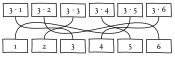
\includegraphics[width=.8\textwidth]{bitmap.png}
  % Beschriftung der Abbildung; in eckigen Klammern der Titel für das
  % Abbildungsverzeichnis
  \caption[Schlecht: Rastergrafik]{Ganz schlechtes Beispiel! (Quelle: \cite[S. 184]{weitz})}
  % frei wählbarer Name für \ref
  \label{fig-bad}
\end{figure}

Abbildung~\ref{fig-better} zeigt im Vergleich eine Vektorgrafik.  Das ist
schon besser, hat aber in den meisten Fällen den Nachteil, dass die Schriften
nicht mit denen Ihrer Arbeit übereinstimmen werden, was unter typographischen
Aspekten sehr unschön ist.\footnote{Das gilt "erst recht" für Tabellen, die
  aus externen Quellen eingefügt werden.}  (Der zugehörige Code in der Datei
\texttt{chap3.tex} zeigt nebenbei, wie man eingefügte Grafiken beschneiden
kann.)

\begin{figure}[!ht]
  \centering
  % es wird nur ein Ausschnitt des Originals eingetzt; die Reihenfolge der
  % vier Werte ist: left bottom right top
  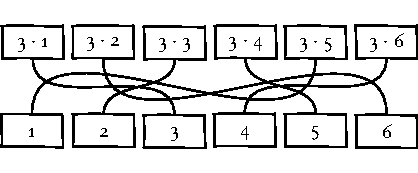
\includegraphics[width=.8\textwidth,trim={0mm 4mm 0mm 4mm},clip]{vector.pdf}
  \caption[Besser, aber noch nicht gut: Vektorgrafik]{Besser, aber nicht optimal (Quelle: \cite[S. 184]{weitz})}
  \label{fig-better}
\end{figure}

Die beste Lösung ist das Erstellen der Grafiken direkt in \LaTeX.  Dazu eignet
sich hervorragend das Paket
\href{https://de.wikipedia.org/wiki/PGF/TikZ}{\textsc{PGF/Ti\textit{k}Z}}, das
nahezu unbegrenzte Möglichkeiten bietet, jedoch eine steile Lernkurve hat.
Dafür ist die mitgelieferte Dokumentation allerdings auch hervorragend.  Als
Einführung kann man auch die Videos in der Playlist
\begin{center}
\url{https://www.youtube.com/playlist?list=PLb0zKSynM2PBbpe9x6LgOZkSCl2yJAOQY}
\end{center}
verwenden.

Diese Vorgehensweise hat zudem den Vorteil, dass man potentiellen Problemen
mit dem Urheberrecht aus dem Weg geht, weil dieses nicht auf eine nach einer
Vorlage selbst erstellte Grafik anwendbar ist.  Nichtsdestotrotz muss aber
auch in diesem Fall die Herkunft benannt werden!

% Zwei ausführliche Beispiele für die Verwendung von TikZ; siehe dazu die
% verlinkte YouTube-Playlist sowie die sehr empfehlenswerte
% TikZ-Dokumentation.
\begin{figure}[!ht]
  \centering
    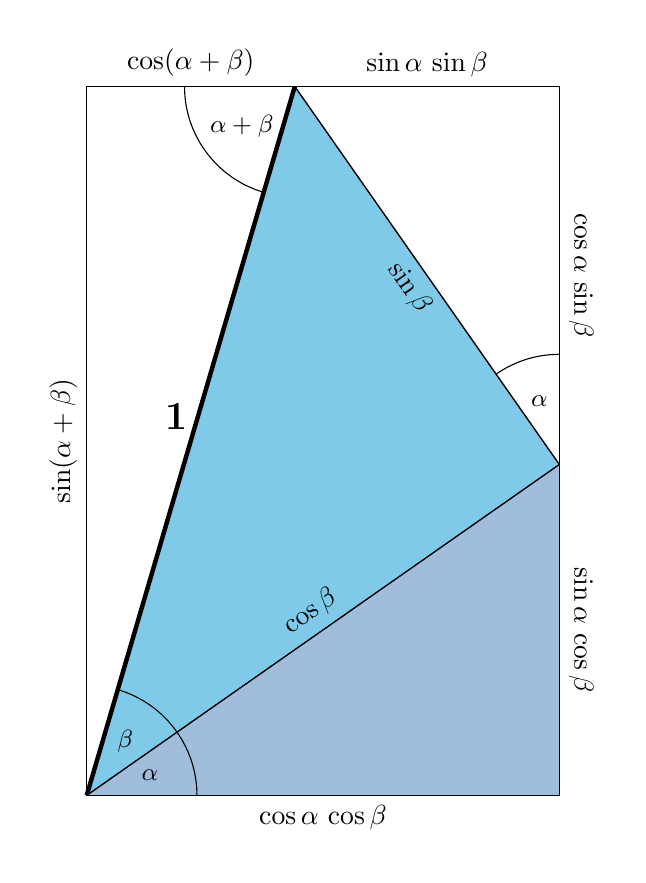
\begin{tikzpicture}[scale=1.5]
      \useasboundingbox (-.5,-.5) rectangle (4.5,6.5);
      \coordinate (O) at (0,0);
      \coordinate (A) at (4,0);
      \coordinate (B) at (4,6);
      \coordinate (E) at (0,6);
      \path[name path=rightEdge] (4,0) -- (B);
      \path[name path=firstHypo] (O) -- ($(O)!1.5!35:(A)$);
      \path[name intersections={of=rightEdge and firstHypo}] (intersection-1) coordinate (C);
      \path[name path=topEdge] (B) -- (E);
      \path[name path=sinEdge] (C) -- ($(C) + (125:5)$);
      \path[name intersections={of=topEdge and sinEdge}] (intersection-1) coordinate (D);
      \fill[haw3] (O) -- (A) -- (C) -- cycle;
      \fill[haw2, fill opacity=.5] (O) -- (C) -- (D) -- cycle;
      \draw (O) rectangle (4,6);
      \draw (O) -- node[sloped, above] {$\cos\beta$} (C);
      \draw (C) -- node[sloped, below] {$\sin\beta$} (D);
      \path (O) -- node[sloped, above] {$\sin(\alpha+\beta)$} (E);
      \path (O) -- node[sloped, below] {$\cos\alpha\,\cos\beta$} (A);
      \path (C) -- node[rotate=180, sloped, above] {$\sin\alpha\,\cos\beta$} (A);
      \path (B) -- node[sloped, above] {$\cos\alpha\,\sin\beta$} (C);
      \path (E) -- node[sloped, above] {$\cos(\alpha+\beta)$} (D);
      \path (D) -- node[sloped, above] {$\sin\alpha\,\sin\beta$} (B);
      \draw (O) -- (C);
      \draw (C) -- (D);
      \draw[ultra thick] (D) -- node[above left, xshift=1mm] {\Large$\mathbf{1}$} (O);
      \draw pic[pic text={\small$\alpha$}, angle radius=1.4cm, draw=black] {angle=A--O--C};
      \draw pic[pic text={\small$\beta$}, angle radius=1.4cm, draw=black] {angle=C--O--D};
      \draw pic[pic text={\small$\alpha+\beta$}, angle radius=1.4cm, draw=black] {angle=E--D--O};
      \draw pic[pic text={\small$\alpha$}, angle radius=1.4cm, draw=black] {angle=B--C--D};
    \end{tikzpicture}
  \caption[Erstes \textsc{Ti\textit{k}Z}-Beispiel]{Mit \textsc{Ti\textit{k}Z} [eigene Grafik nach \parencite[S. 271]{weitz}]}
  \label{fig-tikz}
\end{figure}

% ein Hilfsbefehl für die folgende TikZ-Grafik
\newcommand{\foo}[5]{
  \begin{scope}[xshift=#1cm]
    \begin{scope}[x  = {(1cm,0cm)}, y  = {(0.4cm,0.6cm)}, z  = {(0cm,1cm)}]
      \begin{scope}[canvas is xz plane at y=#4]
        \filldraw[black, fill=#3!70!white] ($(0,0) + (0,#5)$) rectangle ($(0.5,#2) + (0,#5)$);
      \end{scope}
      \pgfmathsetmacro{\z}{#2 + #5}
      \begin{scope}[canvas is xy plane at z=\z]
        \filldraw[black, fill=#3!50!white] (0,#4) -- (0.5,#4) -- ($(0.5,1) + (0,#4)$) -- ($(0,1) + (0,#4)$) -- cycle;
      \end{scope}
      \begin{scope}[canvas is yz plane at x=0.5]
        \filldraw[black, fill=#3!90!white] (#4,#5) rectangle ($(1,#2) + (#4,#5)$);
      \end{scope}
    \end{scope}
  \end{scope}
}

Die Abbildungen \ref{fig-tikz} und~\ref{fig-tikz2} zeigen Beispiele für solche
Grafiken.  Den zugehörigen Quellcode findet man in der Datei
\texttt{chap3.tex}.

\begin{figure}[!ht]
  \centering
    \begin{tikzpicture}[scale=1.5]
      \foreach \i in {1, ..., 16} {
        \pgfmathsetmacro{\shift}{\i / 2}
        \pgfmathsetmacro{\height}{6 / \i}
        \foo{\shift}{\height}{gray}{0}{0}
      }
      \foo{0.5}{3}{haw2}{-1}{0}
      \foo{0.5}{3}{haw3}{-1}{3}
      \foo{1}{3}{haw}{-1}{0}
      \foo{1.5}{1.5}{orange}{-1}{0}
      \foo{2}{1.5}{orange}{-1}{0}
      \foo{2.5}{.75}{purple}{-1}{0}
      \foo{3}{.75}{purple}{-1}{0}
      \foo{3.5}{.75}{purple}{-1}{0}
      \foo{4}{.75}{purple}{-1}{0}
      \foreach \i in {1, ..., 8} {
        \pgfmathsetmacro{\x}{4 + 0.5 * \i}
        \foo{\x}{.375}{brown}{-1}{0}
      }
    \end{tikzpicture}
  \caption[Zweites \textsc{Ti\textit{k}Z}-Beispiel]{Auch mit \textsc{Ti\textit{k}Z} [eigene Grafik nach \parencite[S. 533]{weitz}]}
  \label{fig-tikz2}
\end{figure}

\section{Code}\label{sec-code}

Für die Darstellung von Programmcode wie in Codeblock~\ref{euler} wird in der
Vorlage das Paket \href{https://www.ctan.org/pkg/listings}{\textsc{listings}}
verwendet.

% Verwendung des Pakets "listings" für die Darstellung von Code, der aus der
% externen Datei euler.py gelesen wird
\lstinputlisting[
  % das Paket "kennt" viele gängige Programmiersprachen
  language=Python,
  % Beschriftung
  caption=Eulersches Polygonzugverfahren,
  % frei wählbarer Name für \ref
  label=euler
]{Scripts/euler.py}

In der Datei \texttt{chap3.tex} kann man sehen, wie der Code aus einer
externen Datei eingelesen wird.  Durch diese Vorgehensweise kann man dafür
sorgen, dass auch tatsächlich die aktuelle Version des eigenen Codes verwendet
wird, und man vermeidet potentielle Fehler beim Abtippen.  Man kann den Code
aber auch wie in Codeblock~\ref{kperms} direkt eintippen.

% Verwendung des Pakets "listings" für die Darstellung von Code, der direkt im
% LaTeX-Code eingegeben wird
\begin{lstlisting}[language=Python,caption=Variationen,label=kperms]
def kperm(L, k):
    if k == 0:
        return [[]]
    return [[L[i]]+P for i in range(len(L))
                     for P in kperm(L[:i] + L[i+1:], k-1)]  
\end{lstlisting}

In der Datei \texttt{defs.tex} wird exemplarisch gezeigt, wie man das Aussehen
der Codeblöcke individuell gestalten kann.  Es ist auch möglich, Codeblöcke
wie Abbildungen und Tabellen "gleiten" zu lassen.

Ein Verzeichnis der Codeblöcke kann mit dem Paket \textsc{listings} bei Bedarf
erzeugt werden, wenn Ihre Arbeit sehr viele Codeblöcke enthält.  Umfangreiche
Codeblöcke gehören aber nicht in die Arbeit und auch nicht in den Anhang,
sondern sollten --~ggf. nach Absprache mit der Erstprüferin bzw.\ dem
Erstprüfer~-- auf einem Datenträger zusammen mit der Arbeit eingereicht
werden.
% -*- coding: utf-8 -*-

% Ausgabe des Literaturverzeichnisses; ohne weitere Optionen werden nur die
% Bücher und Artikel ausgegeben, die in der Arbeit auch zitiert werden.
\printbibliography

% markiert den Anfang des Anhangs
\appendix

% ein Kapitel, das nicht numeriert, aber trotzdem ins Inhaltsverzeichnis
% aufgenommen wird
\addchap{Anhang}
% TODO (Daniel): update here se-app
Hier beginnt der Anhang.  Siehe die Anmerkungen zur Sinnhaftigkeit eines
Anhangs in Abschnitt%~\ref{sec-app} auf Seite~\pageref{sec-app}.

Der Anhang kann wie das eigentliche Dokument in Kapitel und Abschnitte
unterteilt werden.  Der Befehl \verb|\appendix| sorgt im Wesentlichen nur für
eine andere Nummerierung.

% neue Seite
\clearpage

% keine Seitenzahl
\thispagestyle{empty}

% keine Nummerierung, keine Aufnahme ins Inhaltsverzeichnis
\section*{Eigenständigkeitserklärung}

% Hier müssen Sie natürlich den Titel der Arbeit sowie Ort und Datum ersetzen:
Hiermit versichere ich, dass ich die vorliegende Bachelorarbeit mit dem Titel
\begin{center}
  \textbf{Performance - Optimierung von Datenbanken}
\end{center}
selbstständig und nur mit den angegebenen Hilfsmitteln verfasst habe.  Alle
Passagen, die ich wörtlich aus der Literatur oder aus anderen Quellen wie
z.\,B. Internetseiten übernommen habe, habe ich deutlich als Zitat mit Angabe
der Quelle kenntlich gemacht.

\vspace{2cm}
% TODO (Daniel): update this here
Hamburg, 21.\ Dezember 1940

\end{document}